\section{Everyone Who Wants to Do Constraint Satisfaction Always Ends in Universal Problems}
% Everyone who wants to do good to the human race always ends in universal bullying.
% - Aldous Huxley
\label{sec:intro-universal}

This second part explores the complexity of the "homomorphism problem" when the data is fixed and the query varies, focusing on "constraint satisfaction problems" and "automatic structures".

\begin{marginfigure}
	\centering
	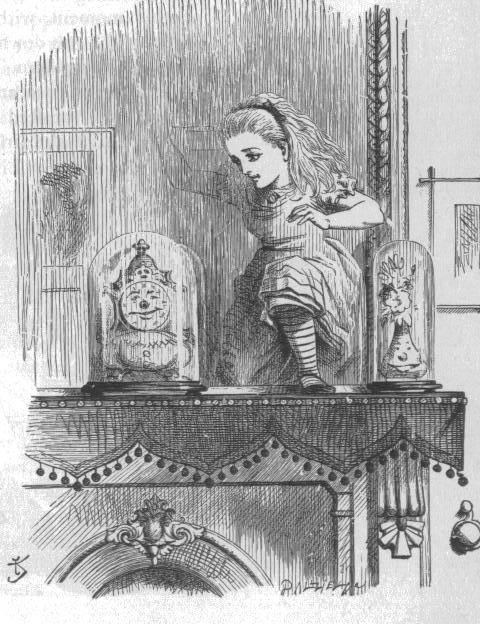
\includegraphics[width=\linewidth]{fig/intro/aliceroom2.jpg}
	\caption{Looking glass room, by John Tenniel.}
\end{marginfigure}

\paragraph*{Constraint Satisfaction Problems.}
Going to the other side, encodings of model-checking problems
as "homomorphism problems" of the form $\textsf{data} \homto^? \textsf{query}$
can be thought of as ``universal problems''---here ``universal'' does not
refer to some form of completeness, but simply to universal quantification.
Notice "eg" that they are anti-monotonic with respect to the data:
for all "structures" $\?A$, $\?A'$ and $\?B$, if $\?A \homto \?B$ and $\?A'$ is a substructure
of $\?A$ then $\?A' \homto \?B$.
Moreover, while problems of the form $\textsf{query} \homto^? \textsf{data}$
can be solved locally---whether a vertex of the data is part of a solution (a "homomorphism") only 
depends on its neighbourhood---, problems $\textsf{data} \homto^? \textsf{query}$ cannot.
For instance, "3-colourability" is a global property of a graph and cannot by gluing local 
solutions. In particular, this implies that fixing the query does not necessarily result in
a drop in the complexity: for instance SAT-solving and "3-colourability" are already "NP"-complete.

However not all of these problems are hard. For example, $2$-colourability is not only polynomial-time,
but can be solved using a greedy algorithm. This begs the question of understanding what
makes a "relational structure" hard for the "homomorphism problem".
This question is not only motivated by theory: constraint logic programming has emerged in the 1980s
with Prolog II and III; today programming languages such as answer-set programming provide an 
efficient was of doing constraint solving.

\begin{figure}
	\centering
	\lstinputlisting[language=Prolog, breaklines=true]{fig/intro/sudoku.lp}
	\caption{
		\AP\label{fig:ex-sudoku-asp}
		A Clingo program (answer-set programming) to solve Sudoku grids.
		Written by Enrico Höschler
		\href{https://ddmler.github.io/asp/2018/07/10/answer-set-programming-sudoku-solver.html}{[source]}.
		Try running it on \url{https://potassco.org/clingo/run/}!
	}
\end{figure}

Answer-set programming can be thought of, albeit caricaturally, as a human-readable
SAT-solver. It deals with variables, relations between these variables,
and logical rules between these variables. These rules take the form
\lstinline|A :- B|, which can be understood as `if $B$, then $A$'.
The right-hand side is parsed conjunctively while the left-hand side is parsed disjunctively:
\lstinline|A, B :- C, D| should be understood as `if $C$ and $D$, then $A$ or $B$'.
\Cref{fig:ex-sudoku-asp} provides
an example of a Clingo program for solving Sudoku grids:
\begin{itemize}
	\item it starts by declaring three types of variables: absissa $x$, ordinates $y$ and entries $x$ (representing a value in the grid), as well as their range;
	\item it introduces a \textsf{sudoku} ternary relation, where $\textsf{sudoku}(x,y,n)$
		represents the fact that entry $(x,y)$ of the grid has value $n$,
		and it says that there should be exactly one value per entry;
	\item it introduces a \textsf{subgrid} relation, saying when too entries
		belong to the same 3*3-square;
	\item finally, it says that any two values on the same column, row or subgrid
		must be different.%
		\footnote{Recall that the left-hand side of rules is understood disjunctively,
		and hence \lstinline|:- A, B| reads as `if $A$ and $B$, then false'.}
\end{itemize}
To solve a specific grid using the program of \Cref{fig:ex-sudoku-asp},
it suffices to add declarations of the form \lstinline|sudoku(4,1,5).|,
where \lstinline|A.| is a shorthand for \lstinline|A :-.|.
This specifies that the cell at position $(4,1)$ has value 5.


Contrary to more classical programming languages, this paradigm does not explain \emph{how} things
should be computed, but \emph{what constraints} the memory/solution should satisfy.
In "homomorphism problems", the "target structure" precisely plays this role of
encoding constraints. For instance, the only constraint for a graph $3$-colouring is that
adjacent vertices must be mapped to distinct colours: this constraint is
reflected in $\clique{3}$ by the fact that the edges of $\clique{3}$ are exactly the pairs
of distinct colours.

The field of \emph{constraint satisfaction problems} precisely aims at classifying the
structures $\?B$ "wrt" to the complexity of the "homomorphism problem" when the
"target structure" is $\?B$. One of the earliest and most impactful result
of the domain as found by Schaefer \cite{Schaefer1978ComplexitySatisfiability},
who proved that such problems are either in "P" or "NP"-complete when the domain of $\?B$
has two elements---this already captures the example of SAT-solving (\Cref{ex:sat-as-hom}) from earlier.
A decade later, Hell and Ne\v{s}et\v{r}il \cite{HellNesetril1990ComplexityColoring}
proved a similar result for undirected graph.
Moreover, in both cases, these dichotomies are effective: given a structure, we can decide if
its "homomorphism problem" is in "P" or is "NP"-complete.
These results, together with the importance of \emph{constraint satisfaction} in computer science
lead Feder and Vardi at the end of the 1990s
to state their infamous \emph{dichotomy conjecture}: ``for any "relational structure" $\?B$,
the "homomorphism problem" with "target structure" $\?B$ is either "P"
or "NP"-complete'' \cite{FederVardi1998ComputationalStructure}.
Despite receiving lots of attention, the conjecture remained wide open for two decades, until
Bulatov \cite{Bulatov2017DichotomyCSPs} and Zhuk \cite{Zhuk2020CSPDichotomy} independently
showed the conjecture to be true.

However not all problems in "P" are complete for this class: some are even simpler and are complete
for "NL" or "L", or even "FOfin"---the class of "first-order definable" "finite structures".
One result that will be of major importance in this thesis is a dichotomy
theorem by Larose and Tesson separating "structures" in "FOfin" from those that are "L"-hard
\cite{LaroseTesson2009UniversalAlgebraCSP}.

\begin{known}
	The field of constraint satisfaction problems classifies "target structures"
	depending on the complexity of their "homomorphism problem".
\end{known}

The second part of this thesis is dedicated to pushing these results to their limit.
These structures are usually always assumed to be "finite@@struct": we want to generalize them
to finitely-presentable\footnote{This assumption is needed for the notion
of computability to make sense.} infinite "structures".

\paragraph*{Automatic structures.}
The end of the XIXth century saw the quest of finding solid foundations
for mathematics. Somewhat surprisingly, this task was much more challenging that expected,
as witnessed by Frege's infamous \emph{Grundgesetze der Arithmetik},
published between 1893 and 1903, presenting an inconsistent set theory due to Russell's paradox.
\todo{finish}

"Automatic structures" are essentially a subclass of "structures" on which the dreams of
the mathematical community holds: given such a "structure" and a "first-order sentence",
we can decide whether it holds on this "structure". These structures can be infinite,
but can be described by finite-state automata, which makes decidability possible.

\begin{known}
	The first-order theory of every "automatic structure" is decidable.
\end{known}

The foremost example of "automatic structure" is "Presburger arithmetic",%
\footnote{See \Cref{ex:presburger}.}
namely the natural number equipped with addition $\tup{\N, +}$.
Sadly, due to "Gödel's incompleteness theorems", there is no single "structure"---let alone an "automatic one@automatic structure"---$\?U$ "st" the sentences of "Zermelo–Fraenkel set theory"
are exactly those true on $\?U$. In fact, Peano's arithmetic, namely natural number with
addition and multiplication $\tup{\N,+,\cdot}$ is not "automatic@@struct".

As a consequence, mathematicians still exist---for better and for worse---as no algorithm
can decide if a given theorem is valid or not.
While "automatic structures" cannot express ``mathematical universes'' serving as
foundations for a universal mathematical theory, they are surprisingly adequate to
express infinite "structures" arising from models of computability.
For instance, the runs of a finite-state automaton is "automatic@@struct"---its nodes
are finite runs of the automaton, and there is a `$a$'-transition from
$\rho$ to $\rho'$ when $\rho' = \rho \transition{a} q'$ for some state $q'$---
since the unfolding of any finite graph is "automatic@@struct".
More generally, the "configuration graph" of any "Turing machine" is "automatic@@struct"!%
\footnote{See \Cref{ex:turing-machine-are-automatic}.}

Hence, we naturally study the "homomorphism problem" when the "input structure"
is allowed to be any "automatic structure". Surprisingly, very little was known about this problem:
the only known result by Köcher states that whether an "automatic graph" is "2-colourable" is undecidable \cite{Kocher2014AutomatischenGraphen}.
This lead us to conjecture that actually most "homomorphism problems" on "automatic structures"
should be undecidable, since $\clique{2}$ is actually somewhat ``simple''.

While the "homomorphism problem" seems quite natural at first glance, a "homomorphism" $f$
from an "automatic structure" $\?A$ to a "finite one@finite structure" $\?B$ does not live
in the same world as $\?A$ and $\?B$, in the sense that it might not be finitely-presentable---its domain is infinite and so, \emph{a priori} require infinite information to be described.
We introduce the notion of "regular homomorphisms", that corresponds to "homomorphisms" that
are finitely-presentable in the same fashion as "automatic structures", and show that
this notion differs from the notion of "homomorphism",
see \Cref{fig:tree-not-2reg-colour,ex:tree-not-2-reg-colourable}.

\begin{marginfigure}
	\centering
	\begin{tikzpicture}
		% ---
% 3-transitive tournament
% ---
\node[vertex, draw=c3, fill=c3, fill opacity=.4] at (0,0) (t3-3) {};
\node[vertex, above=of t3-3, draw=c2, fill=c2, fill opacity=.4] (t3-2) {};
\node[vertex, above=of t3-2, draw=c1, fill=c1, fill opacity=.4] (t3-1) {};
\node[vertex, above=of t3-1, draw=c0, fill=c0, fill opacity=.4] (t3-0) {};

\draw[edge] (t3-0) to (t3-1);
\draw[edge] (t3-1) to (t3-2);
\draw[edge] (t3-2) to (t3-3);
\draw[edge] (t3-0) to[bend left=60] (t3-2);
\draw[edge] (t3-1) to[bend left=60] (t3-3);
\draw[edge] (t3-0) to[bend right=60] (t3-3);
	\end{tikzpicture}
	\caption{
		\AP\label{fig:3-transitive-tournament}
		The "$3$-transitive tournament" $\transitiveTournament{3}$.
	}
\end{marginfigure}
Our first contribution is to show that whether a graph admits a "regular $2$-colouring" is undecidable---see \Cref{thm:k-reg-col-undec}. We then notice that a particular type of
"homomorphism problem" is decidable: for instance, if the "target structure"
is a "transitive tournament". This is best understood on an example: consider the "$3$-transitive 
tournament" depicted in \Cref{fig:3-transitive-tournament}.
A "homomorphism" $f$ from a graph $\?G$ to $\transitiveTournament{3}$ amounts to a function
from the set of vertices of $\?G$ to $\lBrack 0,3\rBrack$ "st"
for any vertices $u$ and $v$, if there is an edge from $u$ to $v$, then
$f(u) \leq f(v)$. It is clear that the existence of such a mapping is in fact equivalent 
to asking that there is no path of length $4$ in $\?G$.
In turn, this property can be expressed by a "first-order formula", and is hence decidable
on "automatic graphs".
More generally, this property can be extended to any "target structure" $\?B$ with the property
that the class of (finite or infinite) "structures" $\?A$ that admit a "homomorphism" to $\?B$
is "first-order definable".
Luckily for us, this class has been well-studied, and is known as the class of "structures"
with "finite duality". In particular, let us cite the result of Larose and Tesson
who proved that any "homomorphism problem" whose "target structure" does not have "finite duality"
must be "L"-hard \cite{LaroseTesson2009UniversalAlgebraCSP}.

The "homomorphism problem" on "automatic structures" 
is undecidable when the "target structure" is a "clique".
Yet it becomes decidable when the target is a transitive tournament.
This contrast leads to conjecture that "finite duality" represents the frontier of decidability for "automatic structures". In \Cref{ch:dichotomy-theorem}, we manage to prove this result, and extend it to "regular homomorphisms".

\begin{contribution}
	We provide a ``dichotomy theorem'' for "homomorphism problems" on "automatic structures":
	for any "finite@@struct" "target structure" $\?B$, the problem
	is either in "NL" or is undecidable. The same holds for "regular homomorphisms".
	Moreover, in both cases, these two problems are decidable precisely when $\?B$ has "finite duality".
\end{contribution}

Since the "configuration graph" of any "Turing machine" is an "automatic graph",
it follows that this dichotomy theorem\footnote{See \Cref{thm:dichotomy-theorem-automatic-structures} for a formal statement.} can be understood
as a variation on "Rice's theorem", that states that any non-trivial
semantical property of a Turing machine is undecidable.
Our dichotomy theorem hence implies the following result.

\begin{contribution}
	Any non-trivial---"ie" "non-first-order definable"---property on the "configuration graph"
	of a "Turing machine" is undecidable, provided that this property can be expressed
	as a "homomorphism problem".
\end{contribution}

One of our motivation for studying this problem was actually originating
in the "$\AUT$/$\REC$-separability problem", which takes as input two "automatic relations"---namely are binary relations over finite words described by "synchronous automata"---and asks if they can be
"separated@@rel" by a "recognizable relation", "ie" a finite union $\bigcup_i K_i \times L_i$
of Cartesian products of "regular languages". 
We prove this problem to be equivalent to the one taking an "automatic graph" and asks
if it has a finite "regular colouring", which amounts to asking
if there exists some $k\in\Np$ for which the graph admits a "regular homomorphism" to
$\clique{k}$. We still don't know whether this problem is decidable, 
even if the result of \Cref{ch:dichotomy-theorem} hint at its undecidability.

When dealing with "regular languages",
separability problems are quite common: a remarkably efficient tool
to prove them decidable is algebraic language theory.
This theory associates to every language a canonical algebra, called "syntactic monoid",
with the property that it is finite if, and only if, the language is "regular@@lang".
Moreover, the language-theoretic and logical properties of the language can be
translated to algebraic properties of this "monoid": more formally, there is a natural
bijection between classes of finite "monoids" and classes of
"regular languages" under mild closure assumptions.

\begin{known}
	Algebraic properties of finite "monoids" correspond to
	language-theoretic and logical properties of "regular languages".
\end{known}

In \Cref{ch:algebra}, motivated by the "$\AUT$/$\REC$-separability problem",
we introduce an algebraic theory for "automatic relations": these algebras are called
"synchronous algebras".
We prove that each finite-word relation admits a "syntactic synchronous algebra",
and that this algebra is finite if, and only if, the relation is "automatic@@rel".

We then prove that classes formed of "these algebras@synchronous algebras" 
are in bijection with the classes of "automatic relations", under some mild closure
assumptions. 

\begin{contribution}
	We extend algebraic language theory to handle relations of finite words
	rather than only languages of finite words.
\end{contribution}

Furthermore, we show that this algebraic theory is relevant, in the following sense.
A "synchronous automaton" encodes a pair (from a binary relation) as
a finite word. This encoding is injective, but not
surjective: not all finite words corresponds to encodings of pairs.
Hence, the semantics of a "synchronous automaton" can be precisely seen
as the semantics of a classical automaton, together with the promise that it will be only
fed inputs that corresponds to valid encodings. In other words,
the behaviour of such an automaton on words that do not correspond to a valid encoding
plays no role whatsoever in its semantics.

This approach is ubiquitous in mathematics, and especially in logics:
for instance, first-order logic over "finite structures" is precisely
defined as first-order logic over all "structures", restricted to "finite structures"!
While being quite natural, this construction fails to preserve most properties of the logics:
first-order logic over all "structures" admits a complete proof system,
but does not when restricted to "finite structures". The model-checking problem
is "coRE"-complete over all "structures", but goes to
"RE"-complete---an incomparable complexity class---for "finite structures".

\begin{contribution}
	We prove that, for any class of "regular languages" satisfying mild closure
	properties, assuming we can decide if a language belongs to this class,
	then we can decide if an "automatic relation" can be written as the restriction
	of a "regular language" in this class with the set of all valid encodings
	of pairs of words.
\end{contribution}

Let us point out that actually, to arrive at this result the notion
of "synchronous algebras" is somewhat intricate. While a more naive definition
exists and makes sense, we show that such a result cannot be proven using this
simpler notion.

This algebraic theory could provide an interesting framework to
study the "$\AUT$/$\REC$-separability problem".
However, the class of "recognizable relations" has some desirable
closure properties we need, but lacks others.
Unfortunately, it implies that proving the decidability of
the "$\AUT$/$\REC$-separability problem" "via" this framework would
be highly non-trivial.

\begin{openproblemintro}
	Can we decide, given two "automatic relations", if they are "separable@@rel"
	by a "recognizable relation"?
\end{openproblemintro}

In summary, this thesis explores two fundamental perspectives on "homomorphism problems":
the first extends the theory of "conjunctive queries" in database theory by adding regular-path
predicates, to capture natural query languages for human-centered graph-shaped data.
It focuses on the problem of query minimization, both in terms of
its total number of atoms, or its tree-width, which is a relevant parameter to
capture the complexity of its evaluation.
The second part focuses on the complexity of problems related to constraint satisfaction
over automatic structures. We show that most \emph{structural} problems, probing the shape of the 
infinite object at hand, are undecidable. In contrast, \emph{language-theoretic} 
problems, dealing with how these infinite structures are represented, remain decidable.